\subsection{Mediciones}

 A continuacion se establecerá como fueron realizadas las mediciones del circuito construido. Los esquemas se elaboraron en proteus y son representativos, se debe hacer caso omiso a la nomenclatura de los componentes. Es importante mencionar que el generador de señales es representado en los esquematicos como una fuente de tension AC.

 Se obviaran las mediciones de tension y corrientes en las resistencias y los transistores FET dada su simplicidad.

\subsubsection{Setup General}
A continuación se vera un acercamiento a las formas de las mediciones a nivel general, las conexiones utilizadas y el espacio de trabajo.

\begin{figure}[H]
    \centering
    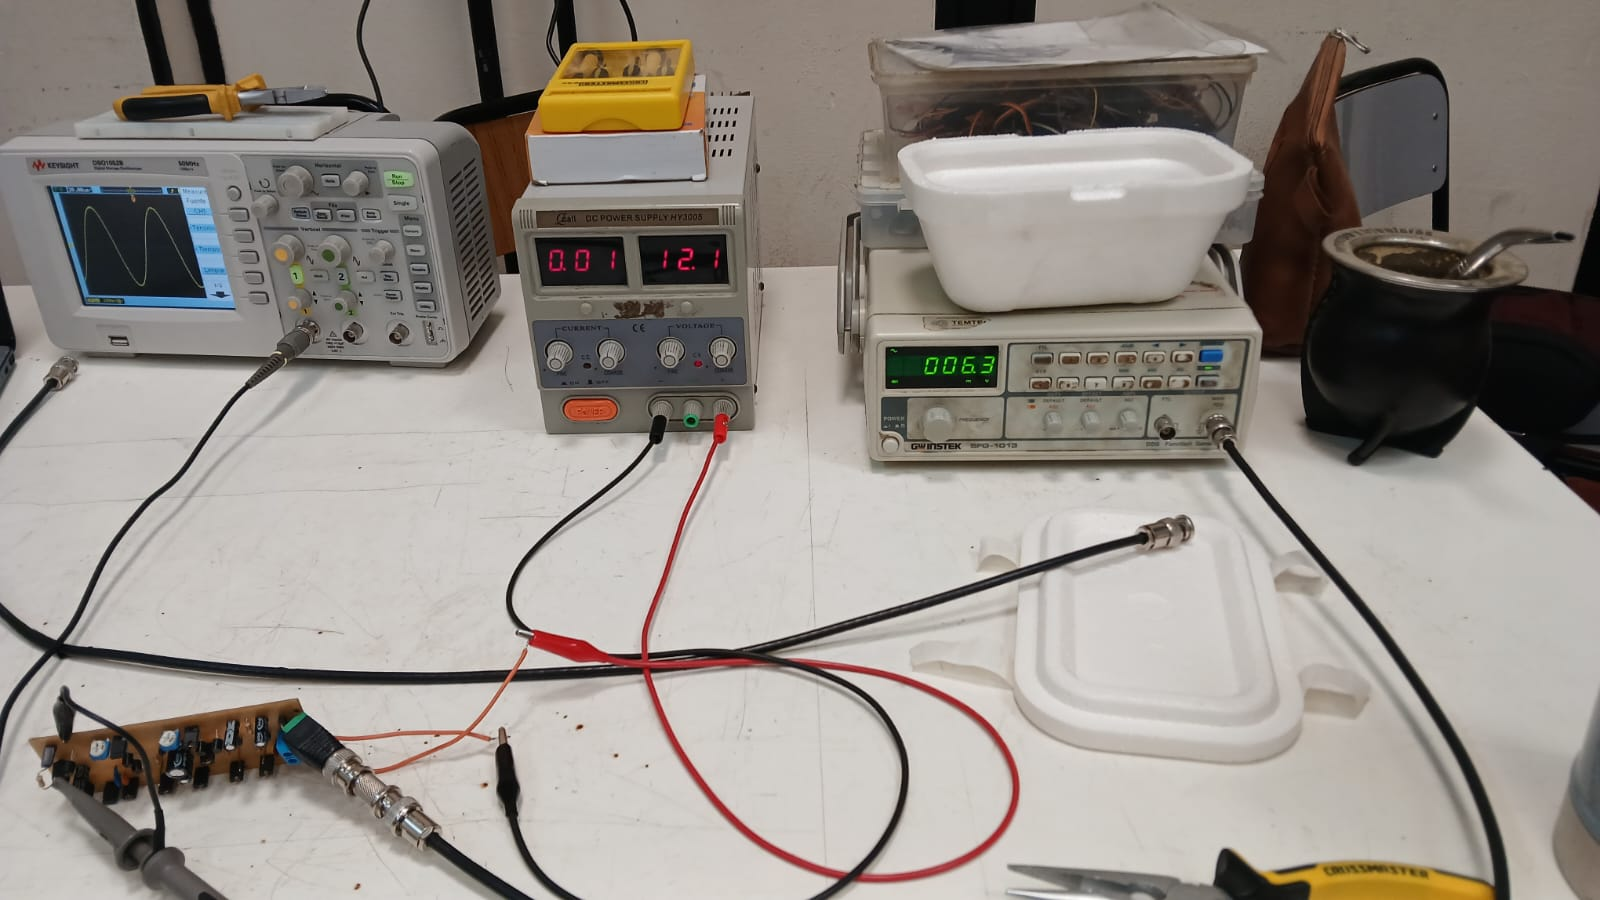
\includegraphics[width=0.65\textwidth]{Imagenes/SetUp.jpeg}
    \caption{Distribucion General}
    \label{fig:DistribucionGeneral}
\end{figure}

\begin{figure}[H]
    \centering
    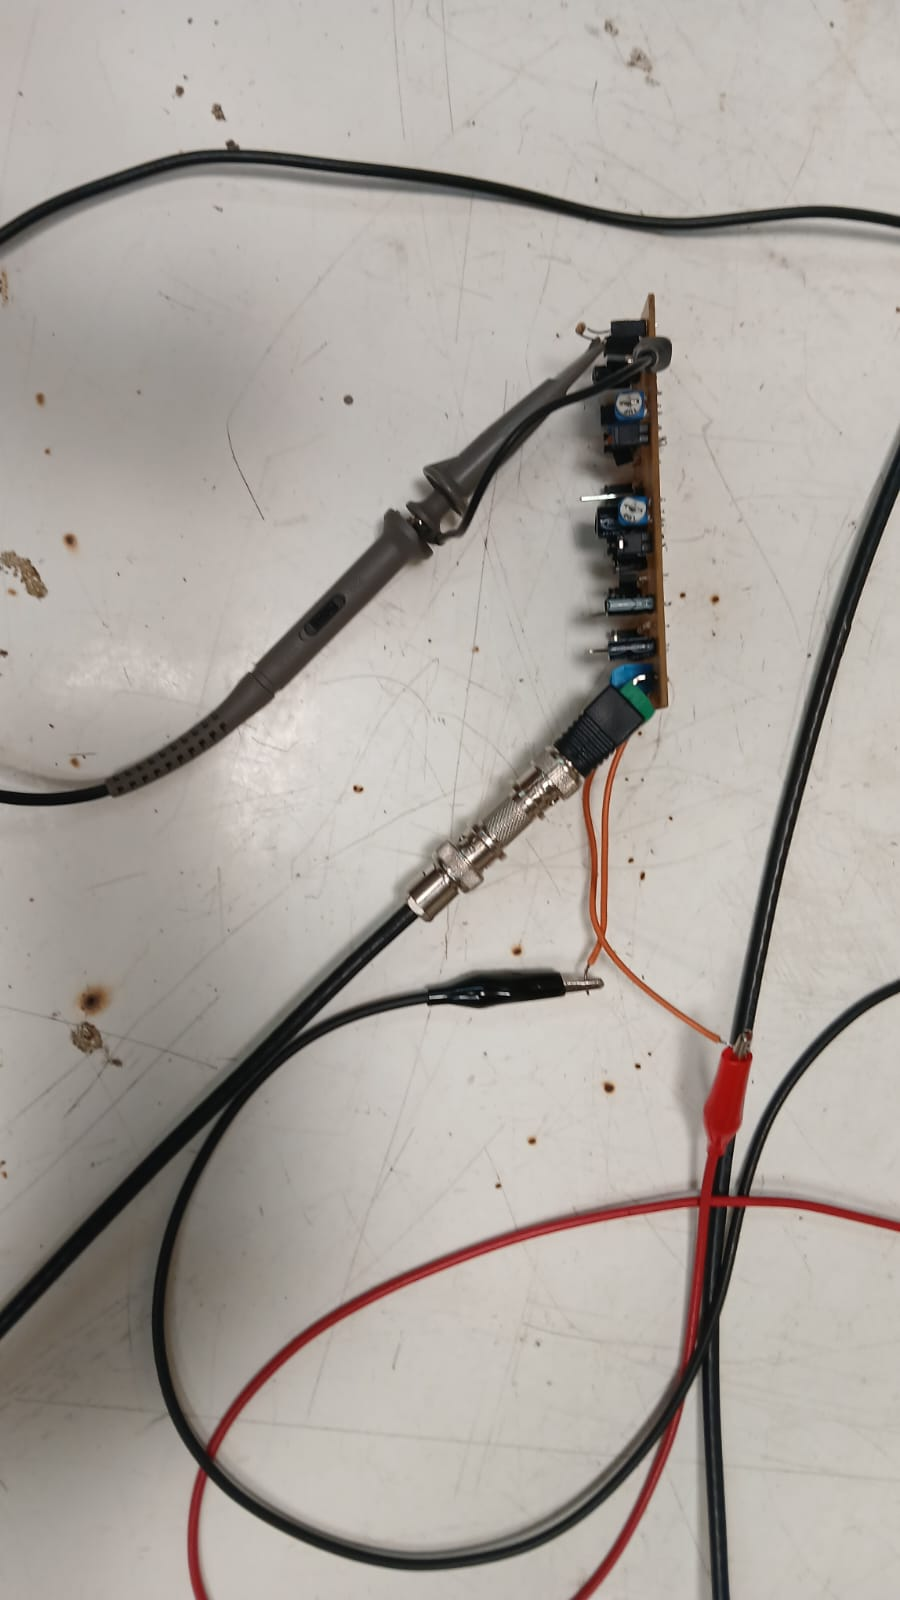
\includegraphics[width=0.35\textwidth]{Imagenes/SetupCercano.jpeg}
    \caption{Conexion a Placa}
    \label{fig:placa}
\end{figure}

A fin de no alargar esta seccion y dadas que muchas de las mediciones tienen distribucione similares, se opto por mostrar la forma representativa esquematica de la distribucion de los instrumentos para cada una de las abarcadas con algunas excepciones.

\subsubsection{Barrido de Amplitud}
Esta medición es realizada en el circuito completo

En esta, las amplitudes de entrada a las configuraciones irán aumentando, esto se realizo incrementando la amplitud de salida del generador de señales.

No se realiza el barrido de amplitud de las etapas por separado ya que se considera que no aportan información útil dado que la ganancia del circuito completo no varia significativamente ante el aumento de tensión en la entrada.

\subsubsection{Barrido del circuito completo}
Su unica distinción es que esta es realizada sin necesidad de modificar el circuito, se mide desde la entrada hasta la ultima etapa

\begin{figure}[H]
    \centering
    % Primera minipage (ocupa el 45% del ancho de la página)
    \begin{minipage}{0.45\textwidth}
        \centering
        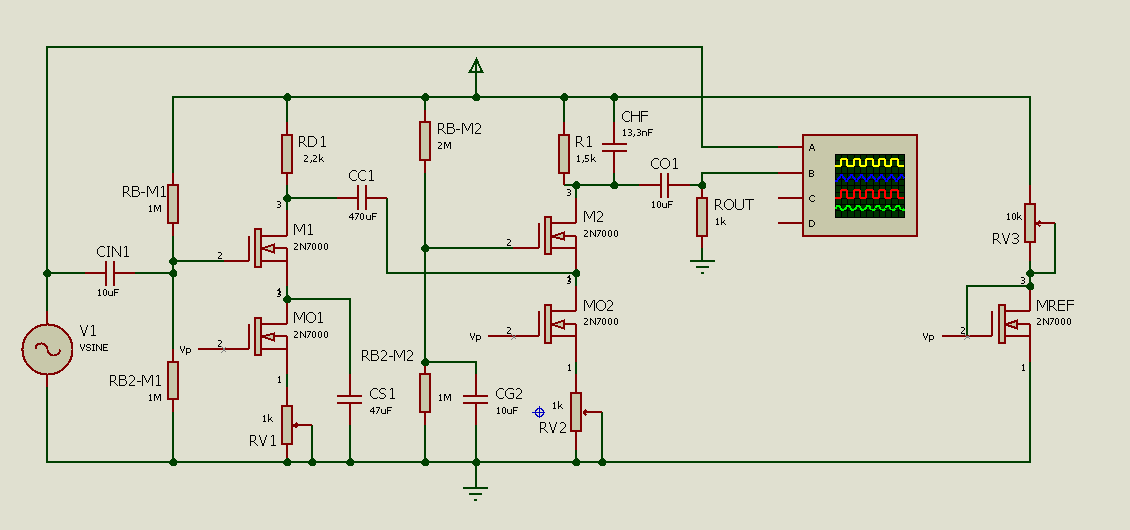
\includegraphics[width=\textwidth]{Imagenes/AvFFTtotal.png} % Ajusta el ancho al de la minipage
        \caption{Representacion esquematica.}
        \label{fig:esquematicoBarCompleto}
    \end{minipage}
    \hfill % Relleno elástico para separar las imágenes
    % Segunda minipage (ocupa el 45% del ancho de la página)
    \begin{minipage}{0.4\textwidth}
        \centering
        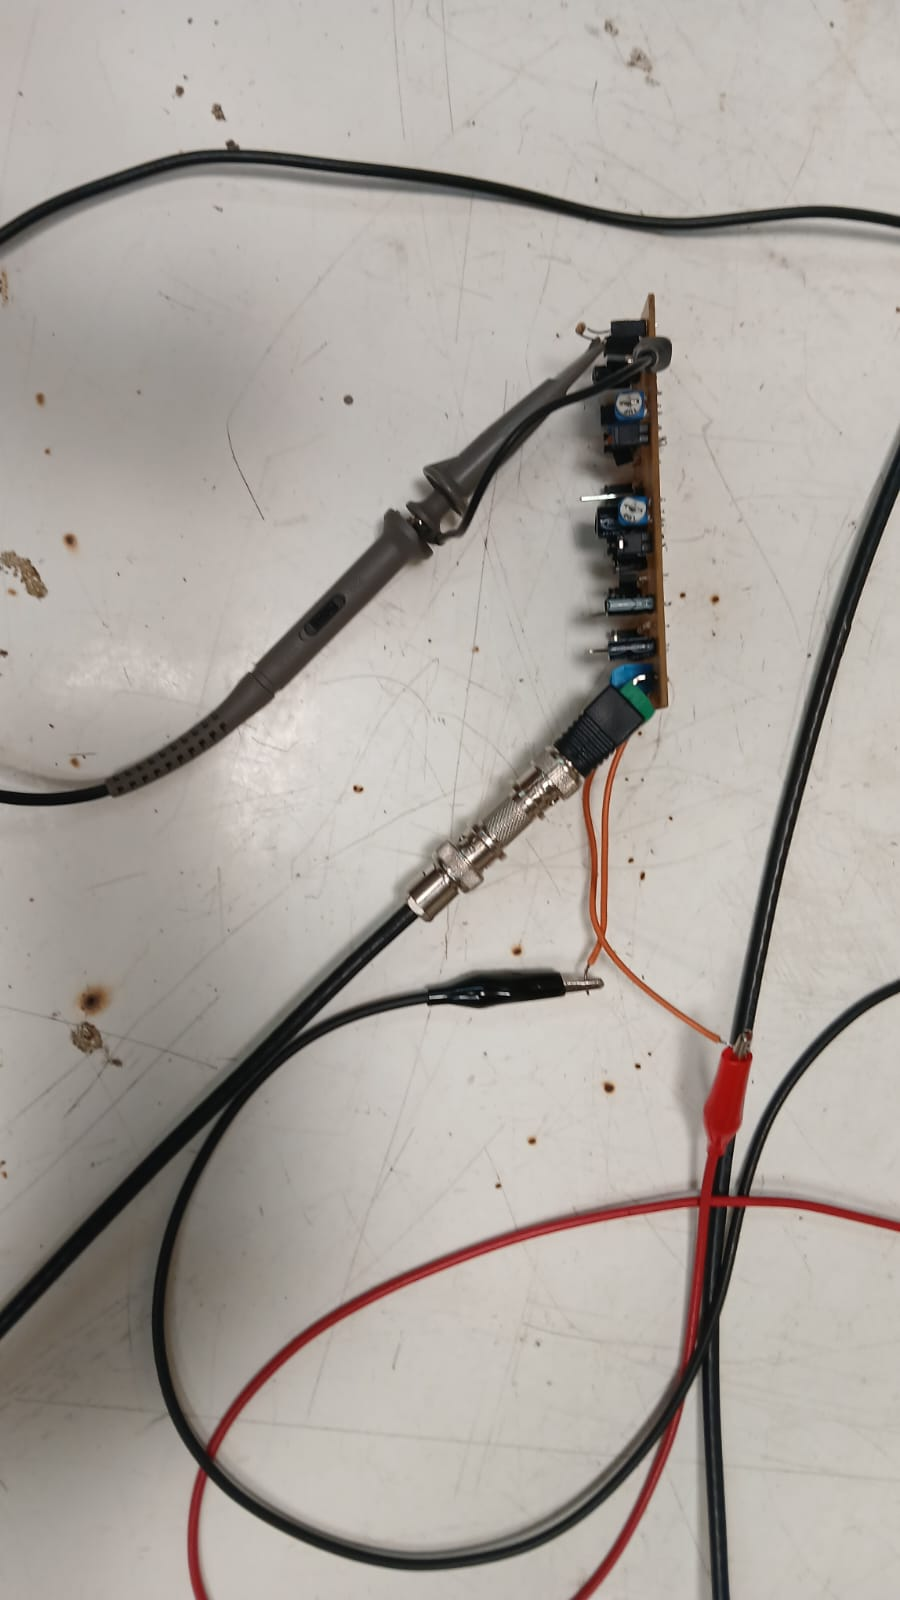
\includegraphics[width=\textwidth]{Imagenes/SetupCercano.jpeg}
        \caption{Imagen de la Medición.}
        \label{fig:medicionBArCompleto}
    \end{minipage}
\end{figure}

\begin{figure}[H]
    \centering
    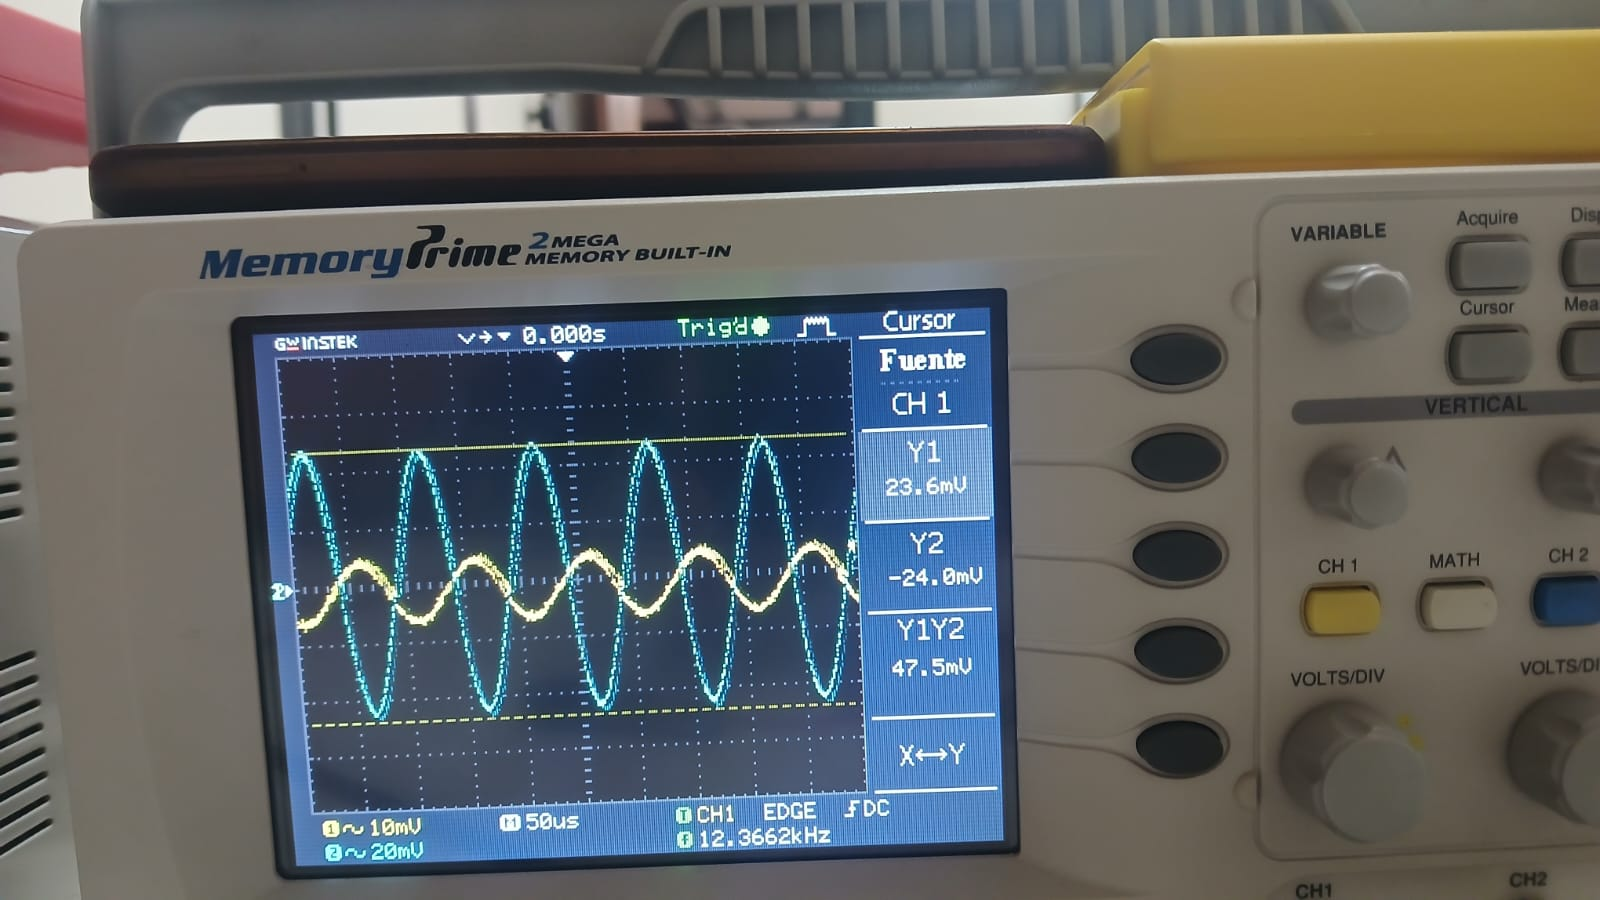
\includegraphics[width=0.8\textwidth]{Imagenes/OSCAvtotal.jpeg}
    \caption{Pantalla del Osciloscopio}
    \label{fig:osciloscopioBarCompleto}
\end{figure}

Se puede ver en \ref{fig:osciloscopioBarCompleto}, dada una entrada proxima a loa 10mVpp, una ganancia cercana a los 9,1 veces la de entrada.

\subsubsection{Barrido de Frecuencia}
Realizada puramente observando el osciloscopio, se fue variando la frecuencia de salida del generador de decada en decada a medida que se realizaban los calculos de ganancia, la amplitud de entrada fue establecida en 5 mV pico a pico. También se Realizaron mediciones sin el CHF acoplado a partir de 1kHz en adelante.

Estas fueron realizadas en 3 configuraciones:
- Etapa 1
- Etapa 2
- Circuito Completo

\paragraph{Barrido de Etapa 1}
Utilizando la punta compensada conectada al osciloscopio se evaluó la tensión de salida de la primer etapa y se realizo el calculo de ganancia.

\begin{figure}[H]
    \centering
    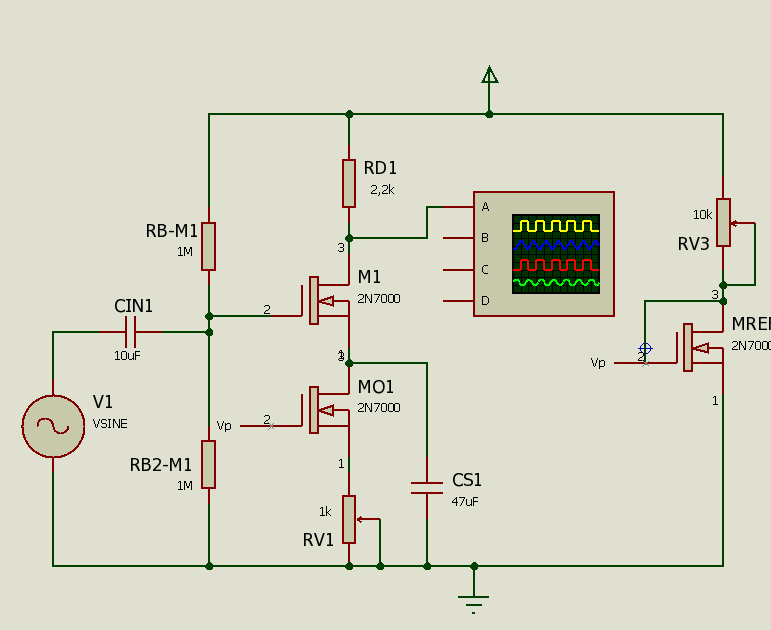
\includegraphics[width=0.6\textwidth]{Imagenes/Av-FFT-Zsc-1.png}
    \caption{Esquematico}
    \label{fig:osciloscopioBArFrec}
\end{figure}

No se realiza la diferenciacion de mediciones con y sin CHF dado que esta no interviene en esta etapa.

\paragraph{Barrido de Etapa 2}
Al igual que con la medicion anterior y en la proxima, se uso la punta compensada conectada al osciloscopio para obtener las mediciones de tension

\begin{figure}[H]
    \centering
    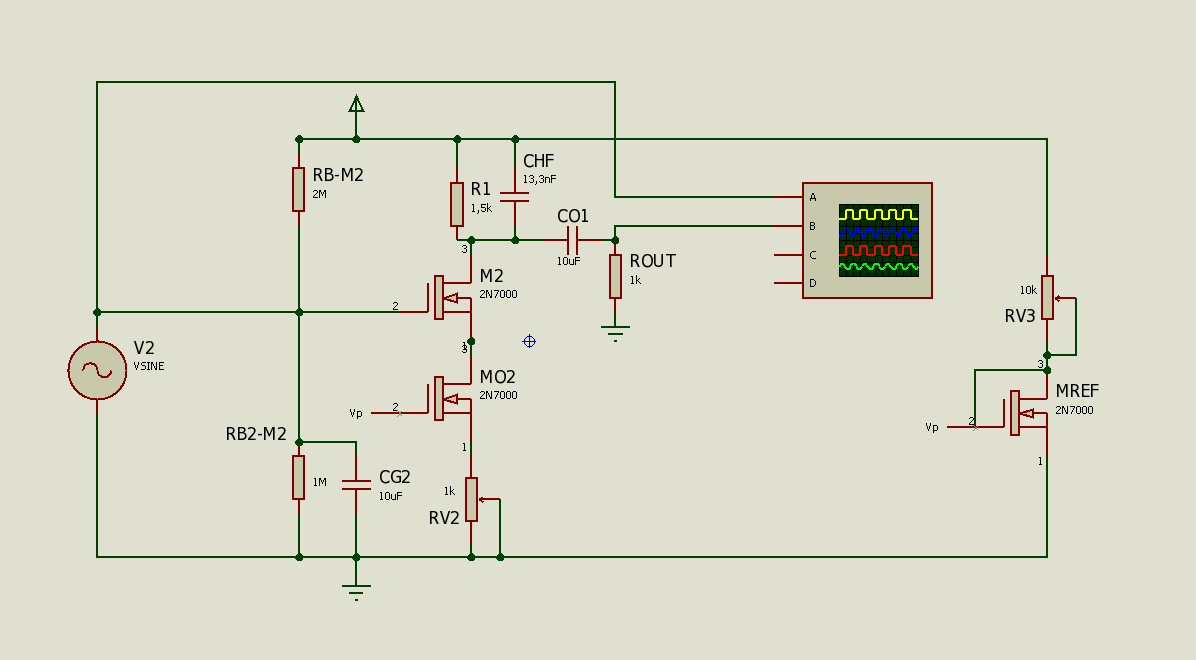
\includegraphics[width=0.6\textwidth]{Imagenes/Av-FFT2.png}
    \caption{Esquematico con CHF}
    \label{fig:osciloscopiofrec12}
\end{figure}

\begin{figure}[H]
    \centering
    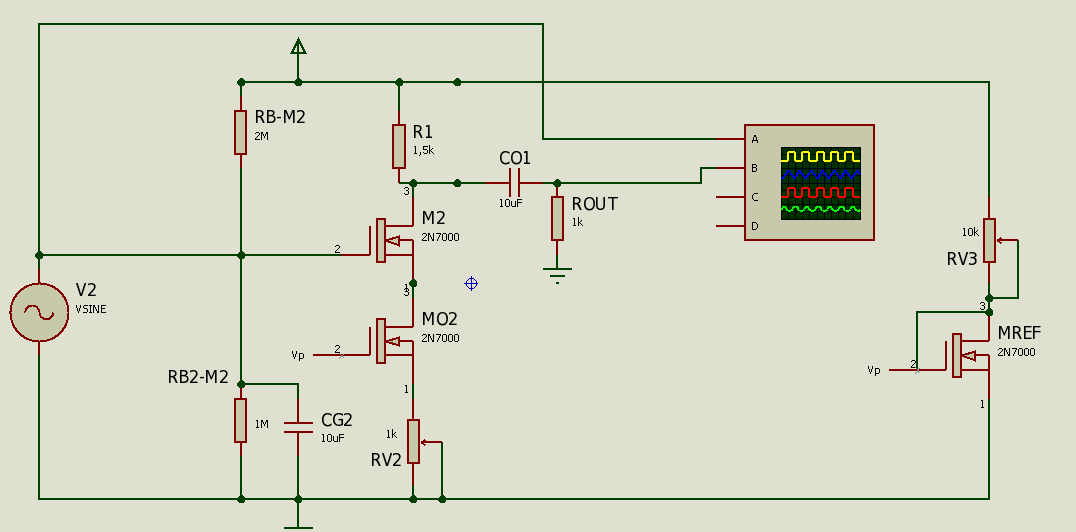
\includegraphics[width=0.6\textwidth]{Imagenes/AvSinCHF2.png}
    \caption{Desacople de CHF}
    \label{fig:esquematicosinCHF2}
\end{figure}

En la medicion vista en la figura \ref{fig:esquematicosinCHF2}, fue realizada desconectando uno de los jumpers de la placa.

\paragraph{Barrido en circuito completo}
Sin casi variaciones, la medicion es reaizada observando la salida del circuito completo.

\begin{figure}[H]
    \centering
    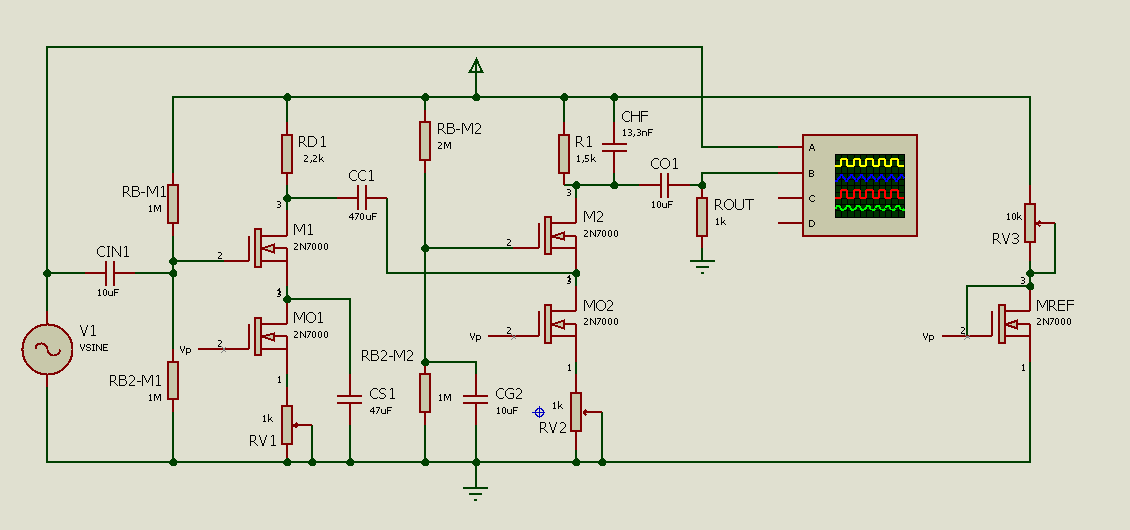
\includegraphics[width=0.6\textwidth]{Imagenes/AvFFTtotal.png}
    \caption{Esquematico del circuito completo}
    \label{fig:Avffttotal}
\end{figure}

\begin{figure}[H]
    \centering
    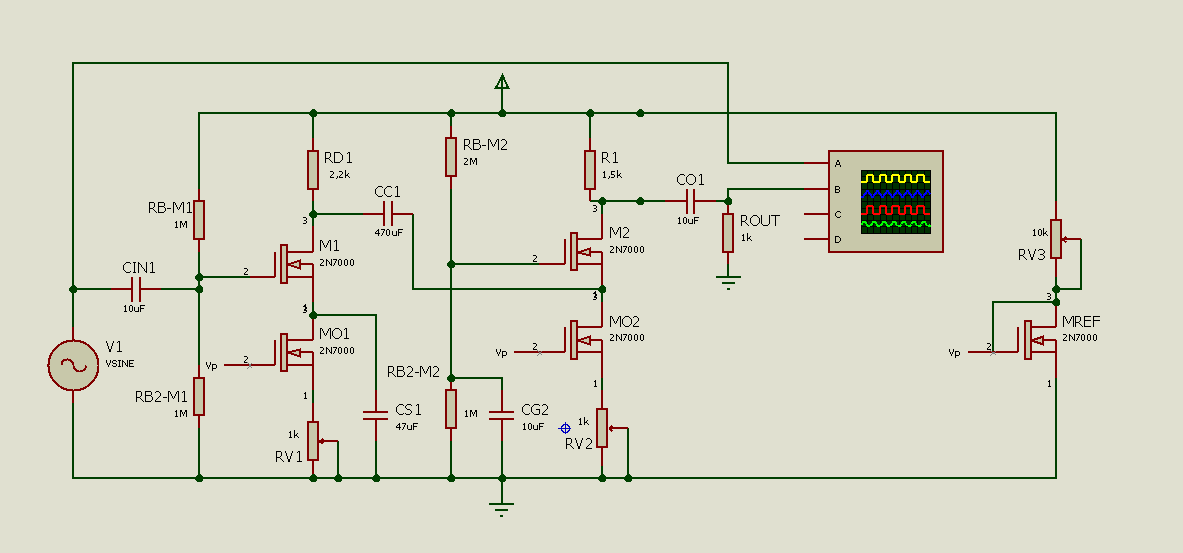
\includegraphics[width=0.8\textwidth]{Imagenes/AvsinCHF.png}
    \caption{Esquematico sin CHF}
    \label{fig:AvffttotalSinCHF}
\end{figure}

\subsubsection{Total Harmonic Distorsion}
Con la misma distribucion dada en el barrido de frecuencia, en este caso se utilizó la funcion de obtener la Transformada Rapida de Fourier (FFT) del osciloscopio para realizar los calculos de THD mediante:

\[
\mathrm{THD} = \frac{\sqrt{V_2^2 + V_3^2 + V_4^2 + \cdots + V_n^2}}{V_1}
\]

Como se dijo anteriormente, se midio en
- Etapa 1
- Etapa 2
- Circuito Completo

\paragraph{FFT de Etapa 1}
Utilizando la punta compensada conectada al osciloscopio se obtuvo la salida de la etapa 1 y se aplico la FFT, una vez impresa en la pantalla se realizaron los calculos pertientes para determinar la THD.

\begin{figure}[H]
    \centering
    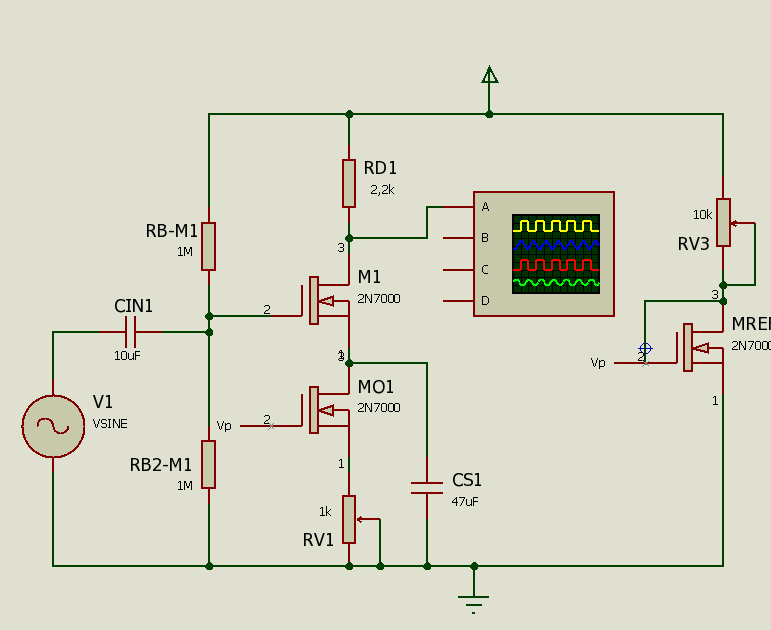
\includegraphics[width=0.8\textwidth]{Imagenes/Av-FFT-Zsc-1.png}
    \caption{Representacion Esquematica}
    \label{fig:esquemaFFT1}
\end{figure}

\begin{figure}[H]
    \centering
    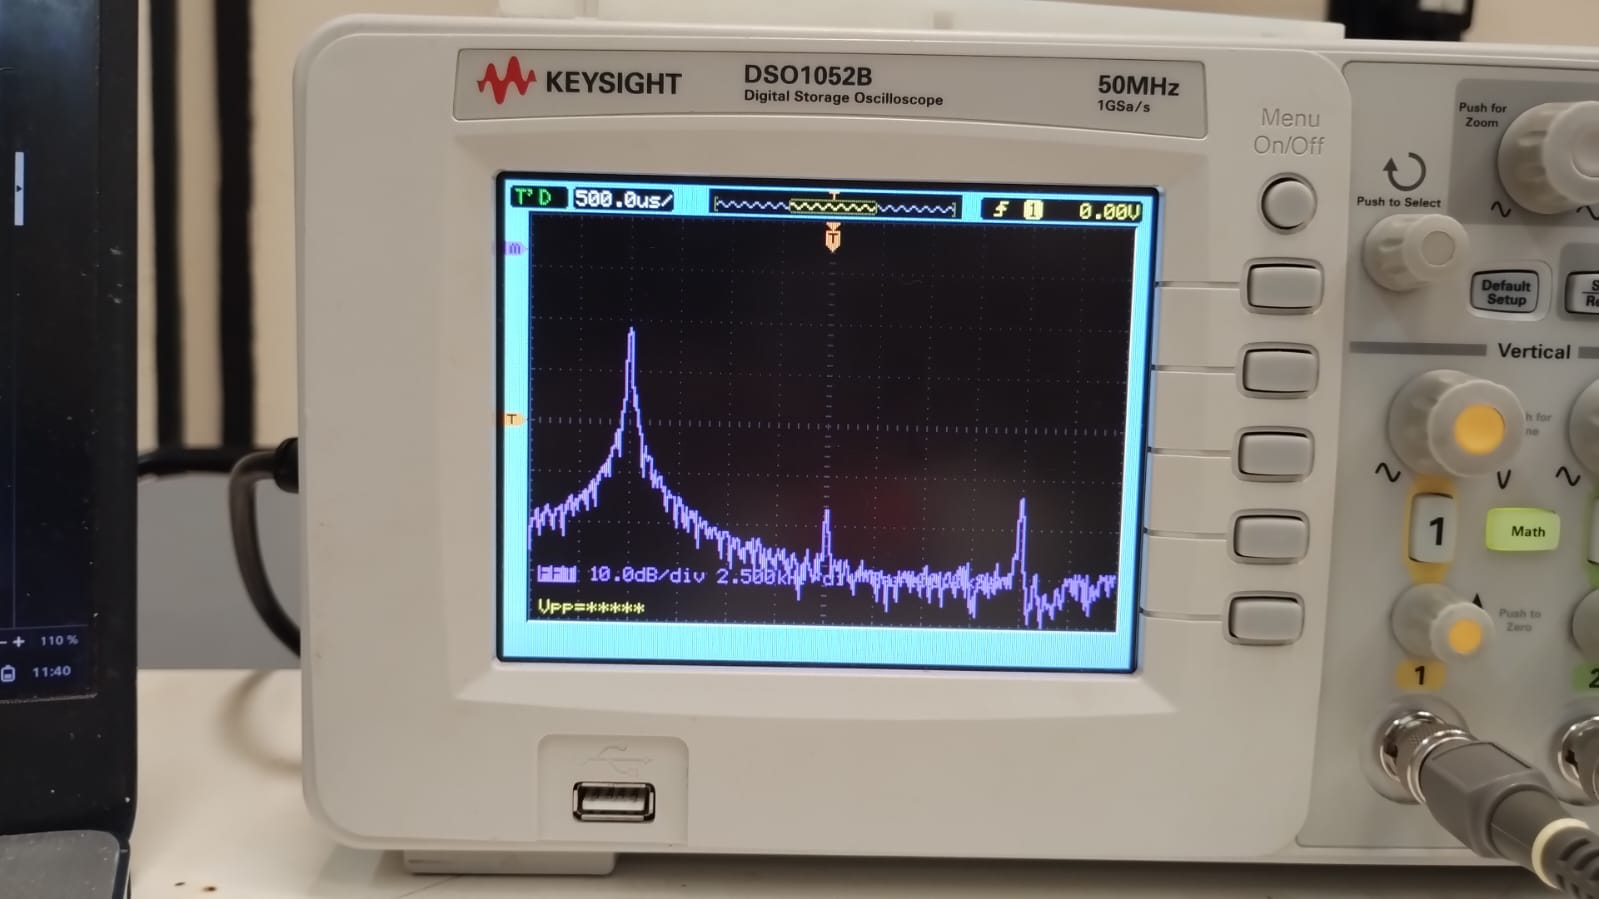
\includegraphics[width=0.8\textwidth]{Imagenes/FFT10kE1.jpeg}
    \caption{Pantalla del Osciloscopio}
    \label{fig:osciloscopioFFT1}
\end{figure}

En la Figura \ref{fig:osciloscopioFFT1}, se muestra la imagen de la FFT de la etapa 1 con una frecuencia de 10KHz con algunos armonicos presentes.

\subsubsection{Barrido de Etapa 2}
Aqui se conectan los jumpers necesarios y se cambia la posicion de la punta a la salida de la etapa 2.

\begin{figure}[H]
    \centering
    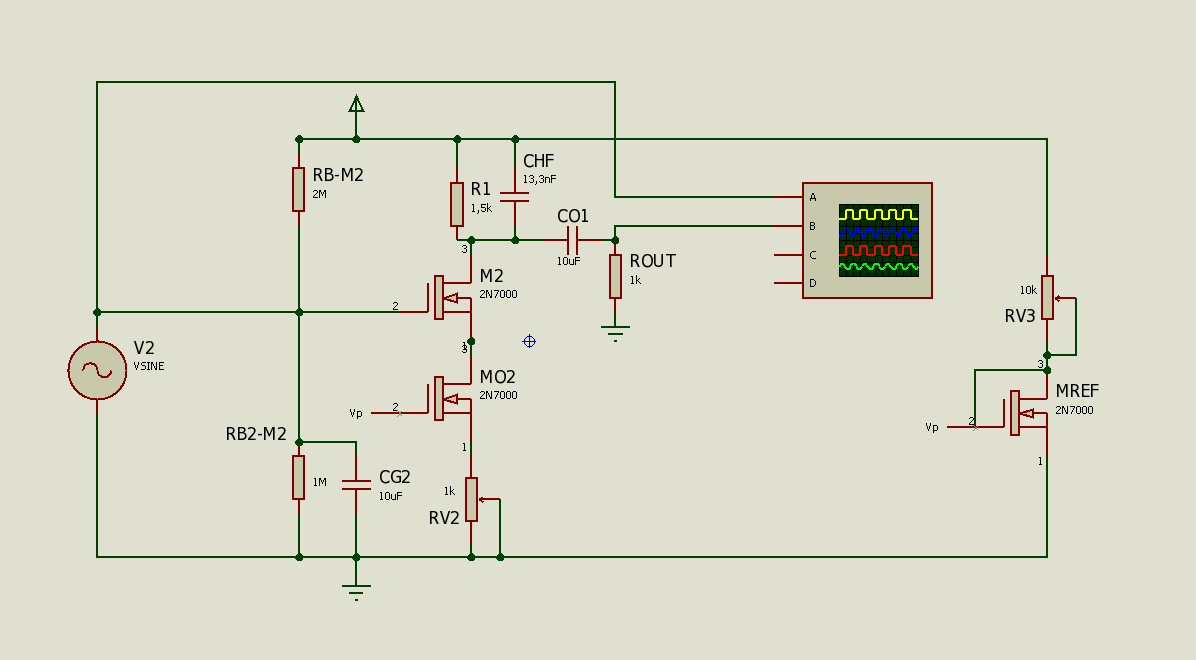
\includegraphics[width=0.8\textwidth]{Imagenes/Av-FFT2.png}
    \caption{Esquemático}
    \label{fig:esquematicofft2}
\end{figure}

\begin{figure}[H]
    \centering
    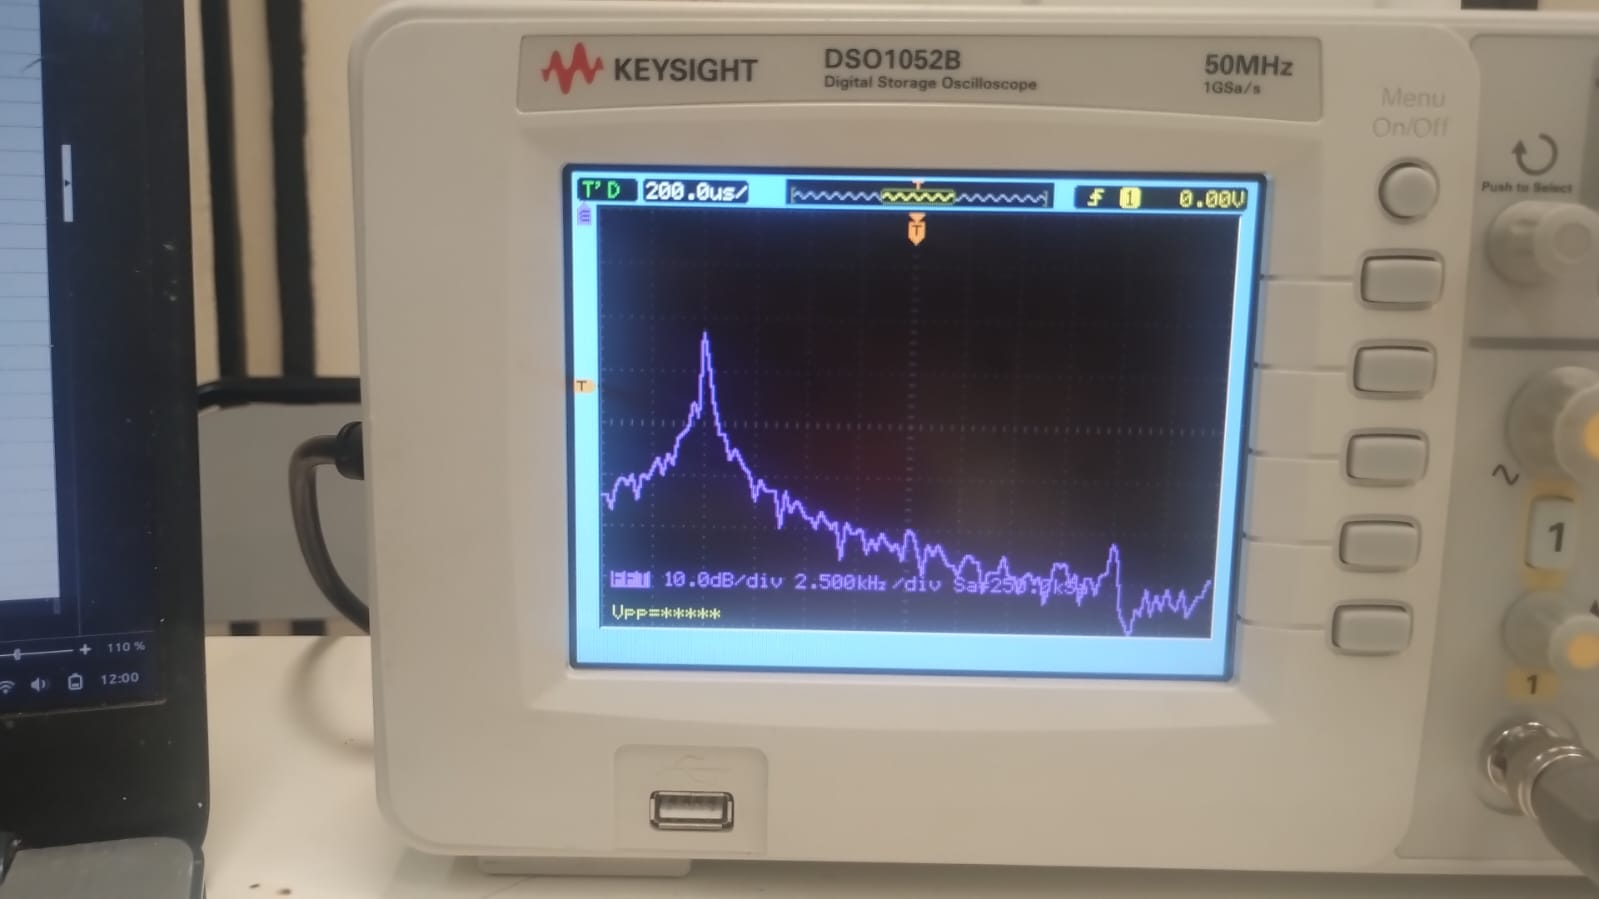
\includegraphics[width=0.8\textwidth]{Imagenes/FFT10kE2.jpeg}
    \caption{Pantalla del Osciloscopio}
    \label{fig:osciloscopioFFT12}
\end{figure}

Se puede ver en \ref{fig:osciloscopioFFT12} la ausencia de armonicos apreciables.

\paragraph{FFT de circuito completo}
Con todos los jumpers conectados, se evalua la FFT del circuito final en la pantalla del osciloscopio 

\begin{figure}[H]
    \centering
    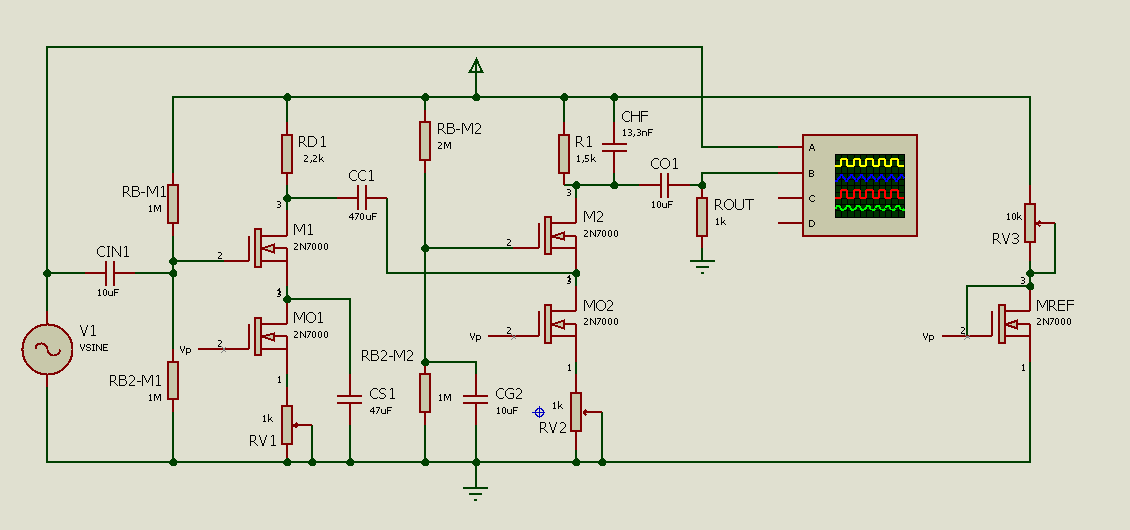
\includegraphics[width=0.8\textwidth]{Imagenes/AvFFTtotal.png}
    \caption{Esquematico}
    \label{fig:EsquematicoFFTCompleto}
\end{figure}

\begin{figure}[H]
    \centering
    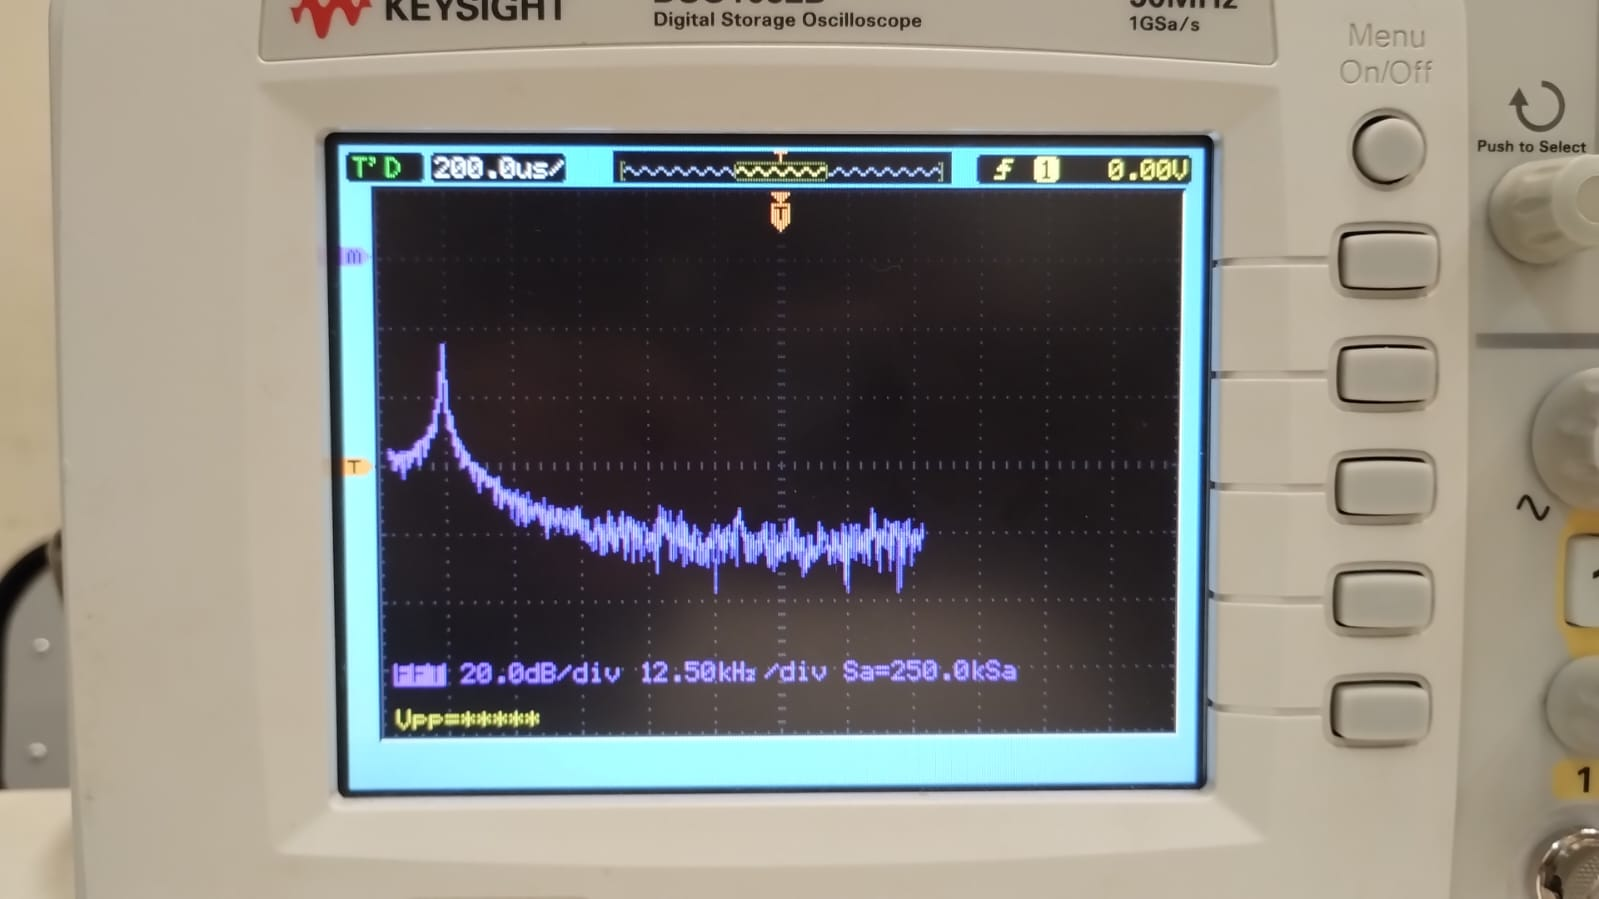
\includegraphics[width=0.8\textwidth]{Imagenes/FFT10kEtotal.jpeg}
    \caption{Pantalla del Osciloscopio}
    \label{fig:osciloscopioFFTCompleto}
\end{figure}

Se puede ver en \ref{fig:osciloscopioFFTCompleto} una ausencia total de armonicos.

\subsubsection{Impedancia De Salida y de Entrada}
A continuacion se vera el método de medicion de las impedancias de salida y de entrada para las siguientes configuraciones

Se midio en:
- Etapa 1
- Etapa 2
- Circuito Completo

\paragraph{Zout}
Para la medicion de impedancia de salida se trabajó en 2 partes para cada configuracion del equipo en pruebas, se midio la tensión a la salida en vacío y con carga conectada. Para todas las mediciones se utilizo una resistencia variable de orden de magnitud similar al esperado en la configuracion en medicion. Una vez obtenidas las mediciones se utilizó la siguiente ecuación:

\[
Z_{\mathrm{out}} = R_L \cdot \left( \frac{V_{\mathrm{vacio}} - V_{\mathrm{carga}}}{V_{\mathrm{carga}}} \right)
\]

Para representar las mediciones se usará como ejemplo la medición de impedancia de salida total.

\begin{figure}[H]
    \centering
    % Primera minipage (ocupa el 45% del ancho de la página)
    \begin{minipage}{0.45\textwidth}
        \centering
        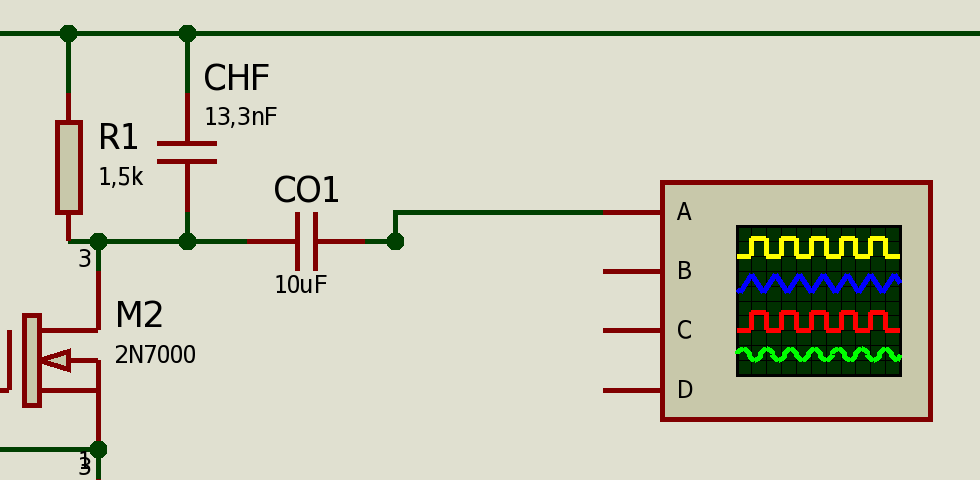
\includegraphics[width=\textwidth]{Imagenes/ZoutTotSinCarga.png} 
        \caption{Esquema de salida sin Carga}
        \label{fig:esquemazoutsincarga}
    \end{minipage}
    \hfill % Relleno elástico para separar las imágenes
    \begin{minipage}{0.45\textwidth}
        \centering
        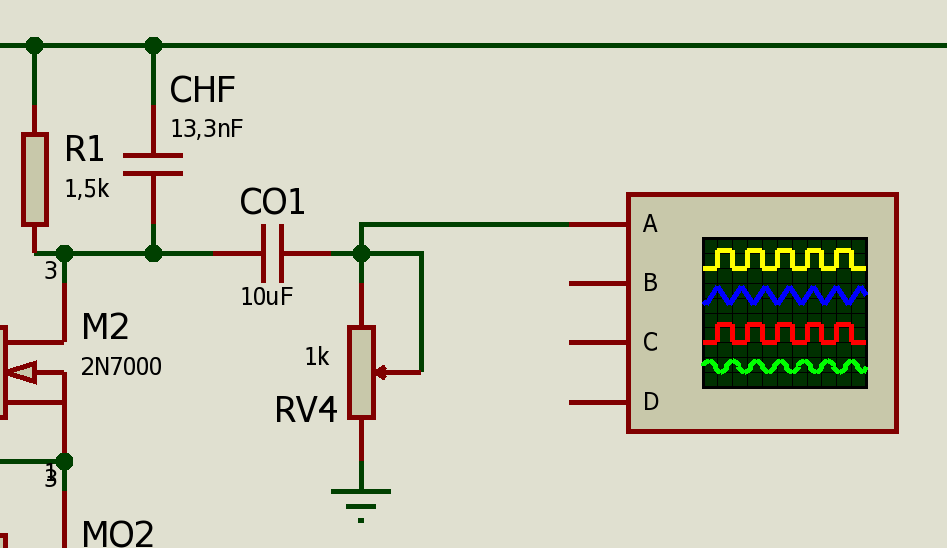
\includegraphics[width=\textwidth]{Imagenes/ZoutTotPreset.png}
        \caption{Esquema de salida cargada.}
        \label{fig:esquemaZoutcargada}
    \end{minipage}
\end{figure}

\paragraph{Zin}
Para la medición de la impedancia de entrada el metodo fue diferente, se inyecto la señal atraves de una resistecnia en serie previa a la entrada de una magnitud similar a la impedancia esperada, dado que, si la tensión luego de la resistencia serie es la mitad que la proporcinaba por el generador, entonces la resistencia es exactamente igual a la Impedancia de entrada de la etapa bajo prueba.

Esto ocurre debido a el metodo de divisior de tension:
\[
V_{\mathrm{circuito}} = \frac{V_{\mathrm{gen}}}{2}
\]

Reemplazando esta igualdad en la ecuación original:

\[
\frac{V_{\mathrm{gen}}}{2} = V_{\mathrm{gen}} \cdot \left( \frac{Z_{\mathrm{in}}}{R_S + Z_{\mathrm{in}}} \right)
\]

Simplificando $V_{\mathrm{gen}}$ en ambos miembros dividiendo por $V_{\mathrm{gen}}$:

\[
\frac{1}{2} = \frac{Z_{\mathrm{in}}}{R_S + Z_{\mathrm{in}}}
\]

Se multiplica cruzado para despejar:

\[
R_S + Z_{\mathrm{in}} = 2 \cdot Z_{\mathrm{in}}
\]

Se resta $Z_{\mathrm{in}}$ en ambos lados:

\[
R_S = 2 \cdot Z_{\mathrm{in}} - Z_{\mathrm{in}}
\]

\[
R_S = Z_{\mathrm{in}}
\]

\[
V_{\mathrm{circuito}} = \frac{V_{\mathrm{gen}}}{2}
\]

Se utilizará de ejemplo la medicion de impedancia de entrada total.

\begin{figure}[H]
    \centering
    % Primera minipage (ocupa el 45% del ancho de la página)
    \begin{minipage}{0.45\textwidth}
        \centering
        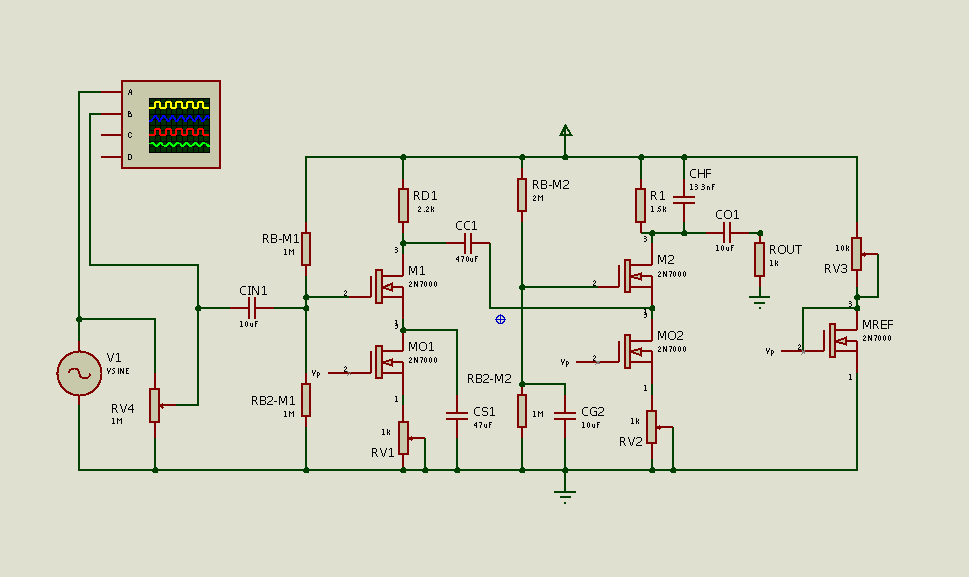
\includegraphics[width=\textwidth]{Imagenes/ZinTotal.png} % Ajusta el ancho al de la minipage
        \caption{Representación esquemática.}
        \label{fig:esquematicpZin}
    \end{minipage}
    \hfill % Relleno elástico para separar las imágenes
    % Segunda minipage (ocupa el 45% del ancho de la página)
    \begin{minipage}{0.45\textwidth}
        \centering
        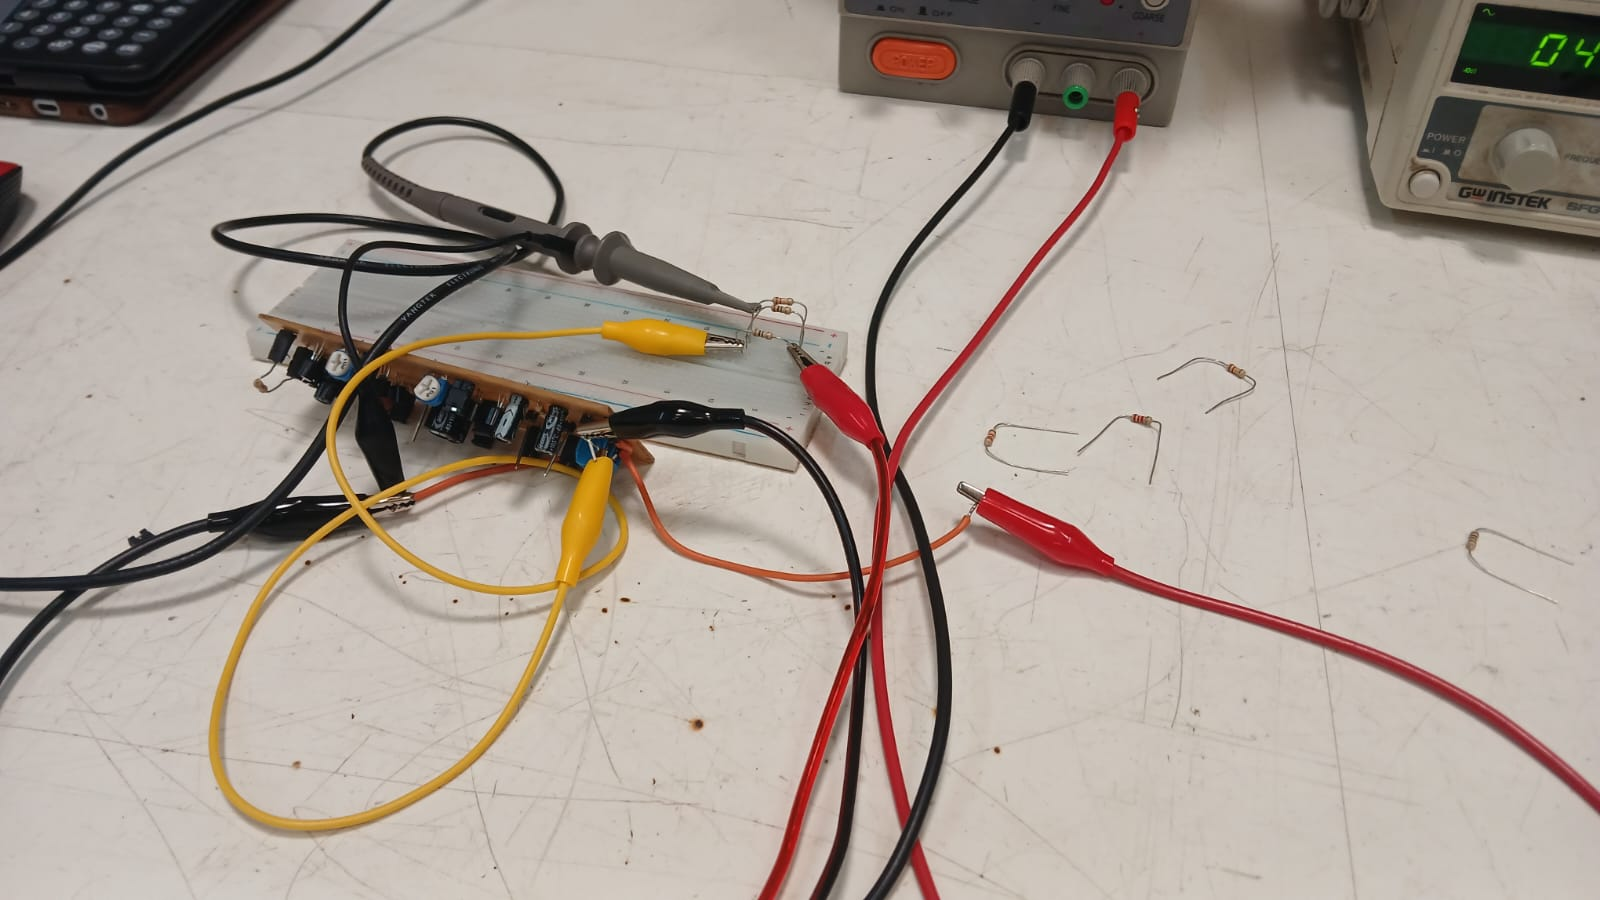
\includegraphics[width=\textwidth]{Imagenes/ZinTotal.jpeg}
        \caption{Setup de la Medición.}
        \label{fig:medicionZin}
    \end{minipage}
\end{figure}

\begin{figure}[H]
    \centering
    % Primera minipage (ocupa el 45% del ancho de la página)
    \begin{minipage}{0.45\textwidth}
        \centering
        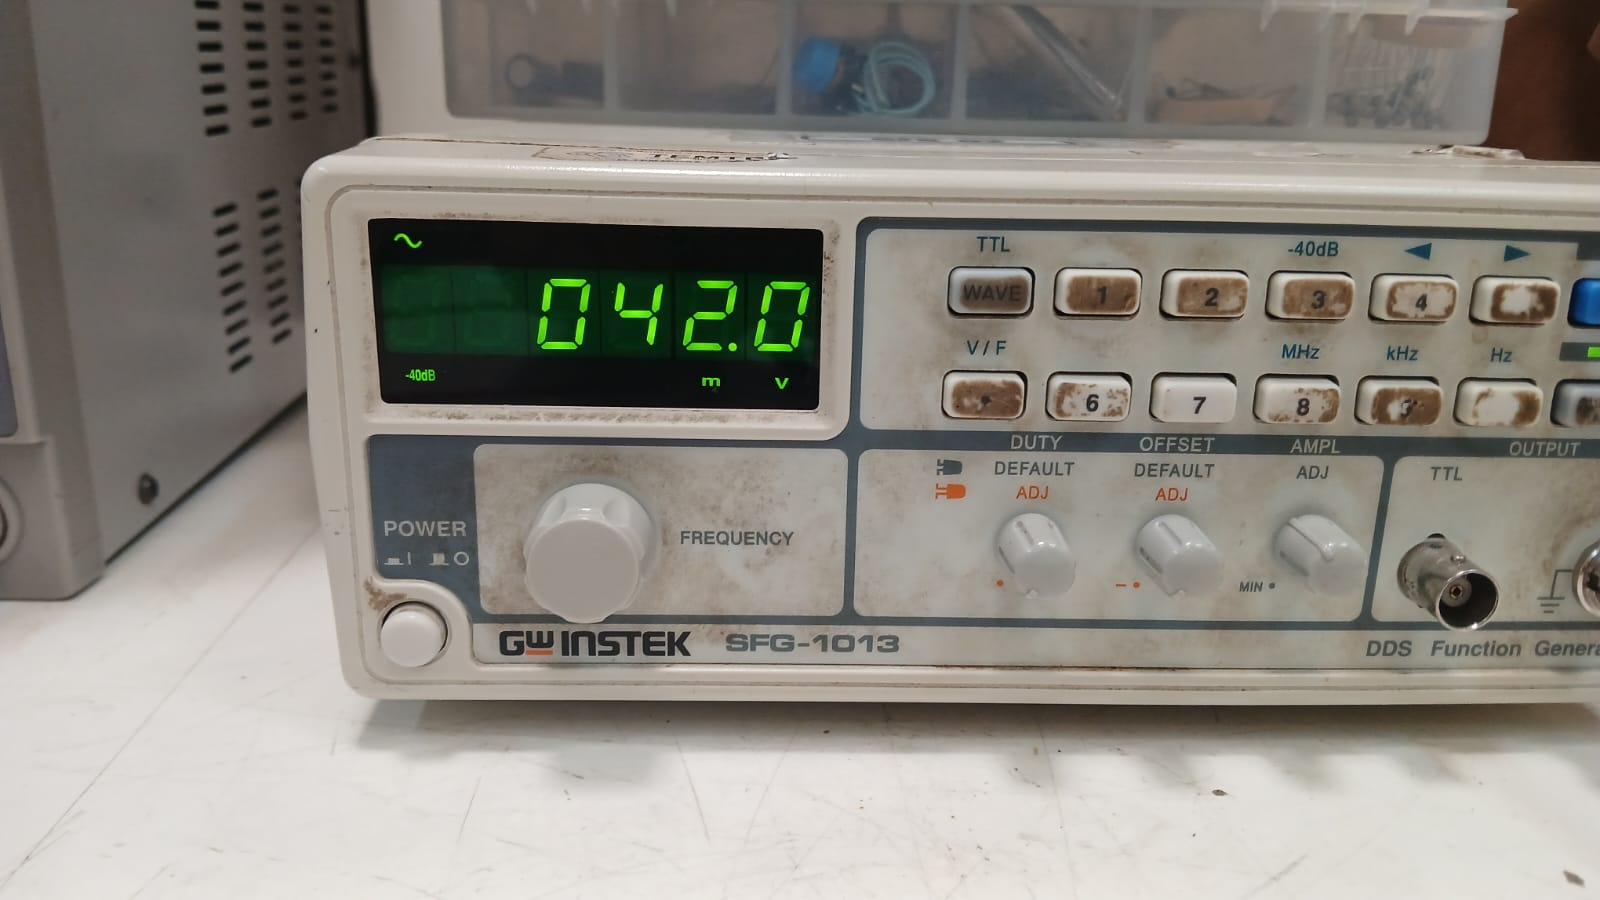
\includegraphics[width=\textwidth]{Imagenes/GenZout.jpeg} % Ajusta el ancho al de la minipage
        \caption{Entrada del Generador.}
        \label{fig:esquematicpZin}
    \end{minipage}
    \hfill % Relleno elástico para separar las imágenes
    % Segunda minipage (ocupa el 45% del ancho de la página)
    \begin{minipage}{0.45\textwidth}
        \centering
        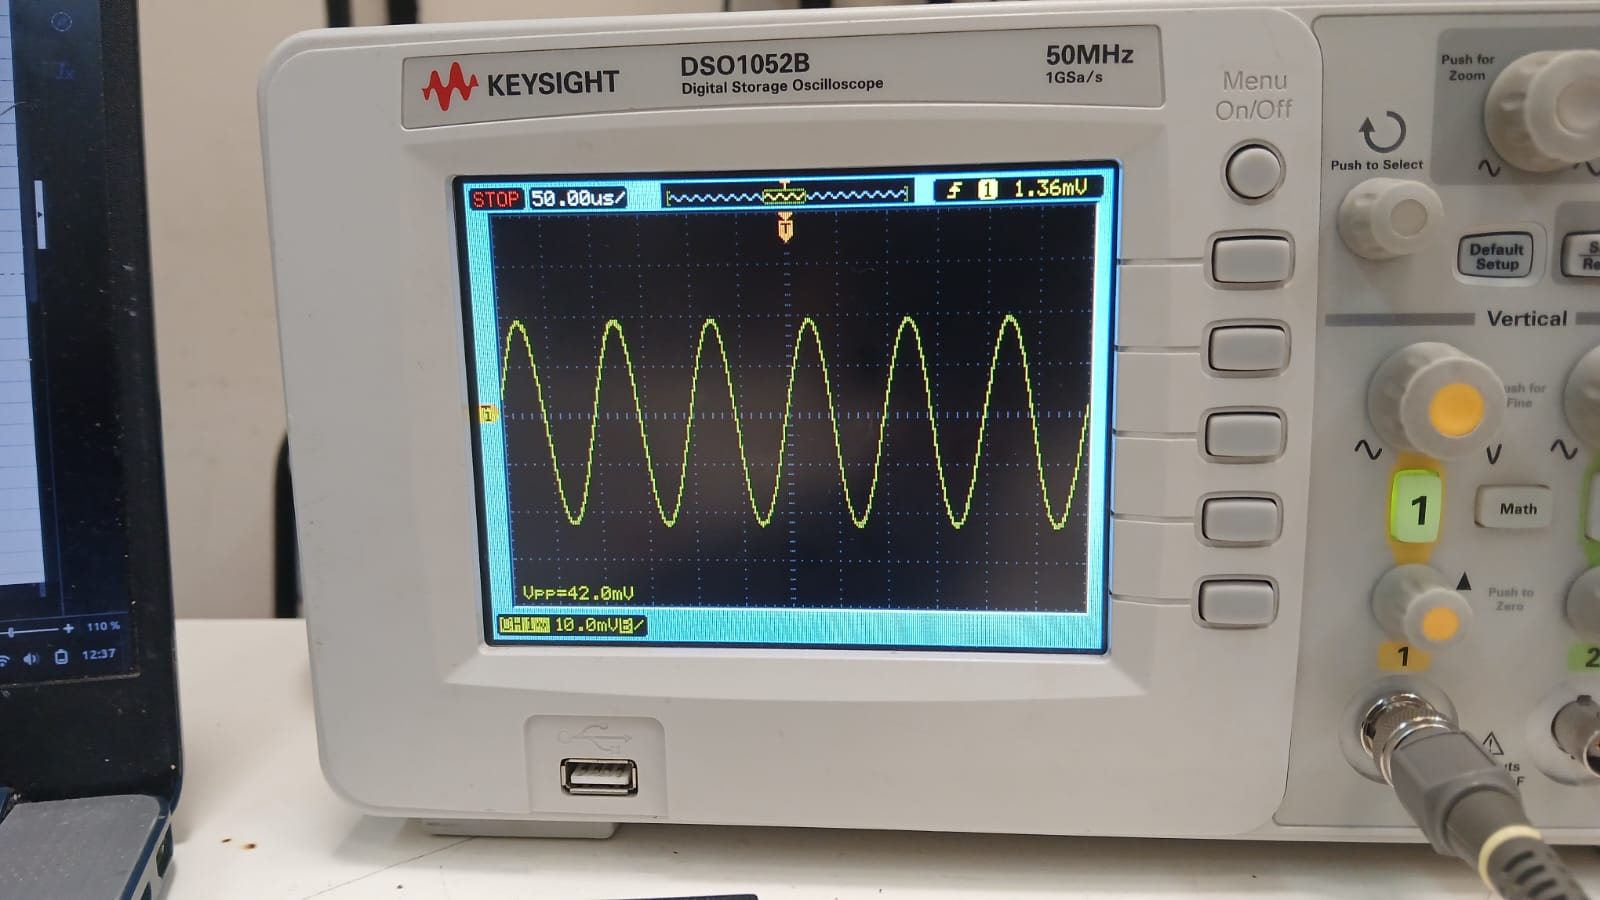
\includegraphics[width=\textwidth]{Imagenes/OscZout.jpeg}
        \caption{Pantalla del Osciloscopio.}
        \label{fig:medicionZin}
    \end{minipage}    
\end{figure}

Se puede ver en la figura \ref{fig:medicionZin} la utilización de combinaciones de resistencias en paralelo para encontrar la impedancia de entrada dada la ausencia de un potenciómetro de magnitud acorde, se fue iterando combinaciones de estas hasta que el osciloscopio de la mitad de la entrada.

Dado que la amplitud del generador es de 42mV, su Vpp es de 82mV, en la pantalla del osciloscopio se deben observar los 42mVpp dispuestos.